\textbf{Note: This is adapted from the document created during the 2024 NVidia Hackathon, see \href{https://docs.google.com/document/d/1x6nGZEiZnAiWBDf20Mcbwbob9a6GMbx3ZpT_huUVZF4/edit?usp=sharing}{original here}.
}
\subsection{Profiling a simple script with NSight}

For profiling, in addition to usual DESC dependencies, you will need \textbf{nvtx} which you can install using pip,

\begin{minted}[fontsize=\footnotesize]{bash}
pip install nvtx
\end{minted}

Here’s a simple test script that we use for profiling equilibrium solve.

\begin{minted}[fontsize=\footnotesize]{python}
from desc import set_device
set_device("gpu")
import numpy as np

from desc.equilibrium import Equilibrium
from desc.geometry import FourierRZToroidalSurface
from desc.objectives import (
    ObjectiveFunction,
    ForceBalance,
    get_fixed_boundary_constraints,
)
from desc.optimize import Optimizer
from desc.plotting import plot_1d, plot_section, plot_surfaces
from desc.profiles import PowerSeriesProfile
import sys
import nvtx

with nvtx.annotate("surface 2D Init"):
    surface_2D = FourierRZToroidalSurface(
        R_lmn=np.array([10, -1]),                                                    
        Z_lmn=np.array([1]),
        modes_R=np.array([[0, 0], [1, 0]]),                                                                 
        modes_Z=np.array([[-1, 0]]),
        NFP=5,                                                                             
    )                       
with nvtx.annotate("Equilibrium Init"):
    eq = Equilibrium(
        surface=surface_2D,
        sym=True,
        L=int(sys.argv[1]),
        M=int(sys.argv[1]),
        N=int(sys.argv[1]),
        L_grid=2*int(sys.argv[1]),
        M_grid=2*int(sys.argv[1]),
        N_grid=2*int(sys.argv[1]),
    )
with nvtx.annotate("Objectives"):
    objective = ObjectiveFunction(ForceBalance(eq=eq))
with nvtx.annotate("Constraints"):
    constraints = get_fixed_boundary_constraints(eq=eq)
with nvtx.annotate("optimizer"):
    optimizer = Optimizer("lsq-exact")
with nvtx.annotate("solve"):
    eq, solver_outputs = eq.solve(
        objective=objective, constraints=constraints, optimizer=optimizer, maxiter=10, ftol=0, gtol=0, xtol=0, verbose=3
    )
\end{minted}

We run this script with NSight on the Della cluster. 

\begin{minted}[fontsize=\footnotesize]{bash}
module purge
module load anaconda3/2024.6
conda activate desc-env
nsys profile --trace=nvtx python3 <test_script.py> 4  > trace0.out 
\end{minted}


Of course for running this on GPU, you will need to ask for a GPU in your slurm. For more slurm options, check \href{https://researchcomputing.princeton.edu/support/knowledge-base/slurm}{Princeton Research cluster page}.

\begin{minted}[fontsize=\footnotesize]{bash}
#!/bin/bash
#SBATCH --job-name=profile        # create a short name for your job
#SBATCH --nodes=1                # node count
#SBATCH --cpus-per-task=32        # cpu-cores per task (>1 if multi-threaded tasks)
#SBATCH --mem=64G         # memory per cpu-core (4G is default)
#SBATCH --time=00:15:00          # total run time limit (HH:MM:SS)
#SBATCH --gres=gpu:1
#SBATCH --constraint=gpu80

module purge
module load anaconda3/2024.6
conda activate desc-env

nsys profile --trace=nvtx,cuda,cusolver --output=your-name-for-the-report --force-overwrite=true python test_script.py 12
\end{minted}

Here, \textbf{--constraint=gpu80} is optional (asks a GPU with 80GB memory). \textbf{--trace=nvtx,cuda,cusolver} part optionally traces cuda and cusolver activities, for example QR or SVD calls can be seen with these settings. \textbf{--output} is used for giving a name for the report. \textbf{--force-overwrite} is used to overwrite the existing file (note that for the overwrite to happen successfully, you should close the file from Nsight systems, which we will talk in shortly). For more details on Nsight options, check \href{https://docs.nvidia.com/nsight-systems/UserGuide/}{NVidia page}.

To run the NSight GUI, you must log on the Della visual node. 
\begin{figure}[H]
    \centering
    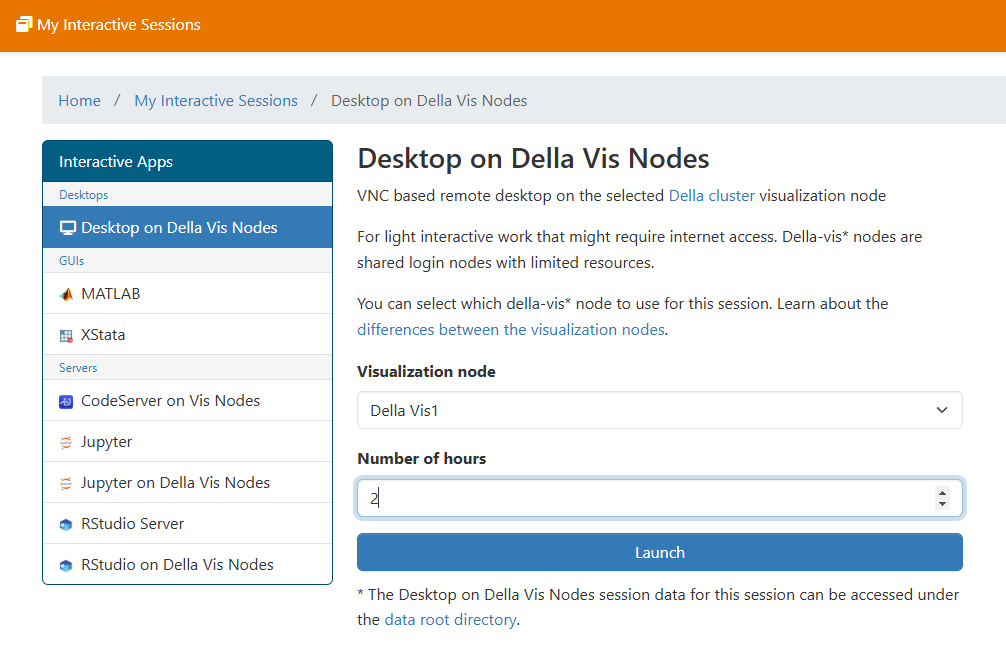
\includegraphics[width=0.5\linewidth]{figures/della-visnode.png}
\end{figure}

Then, open the Nsight systems software,
\begin{figure}[H]
    \centering
    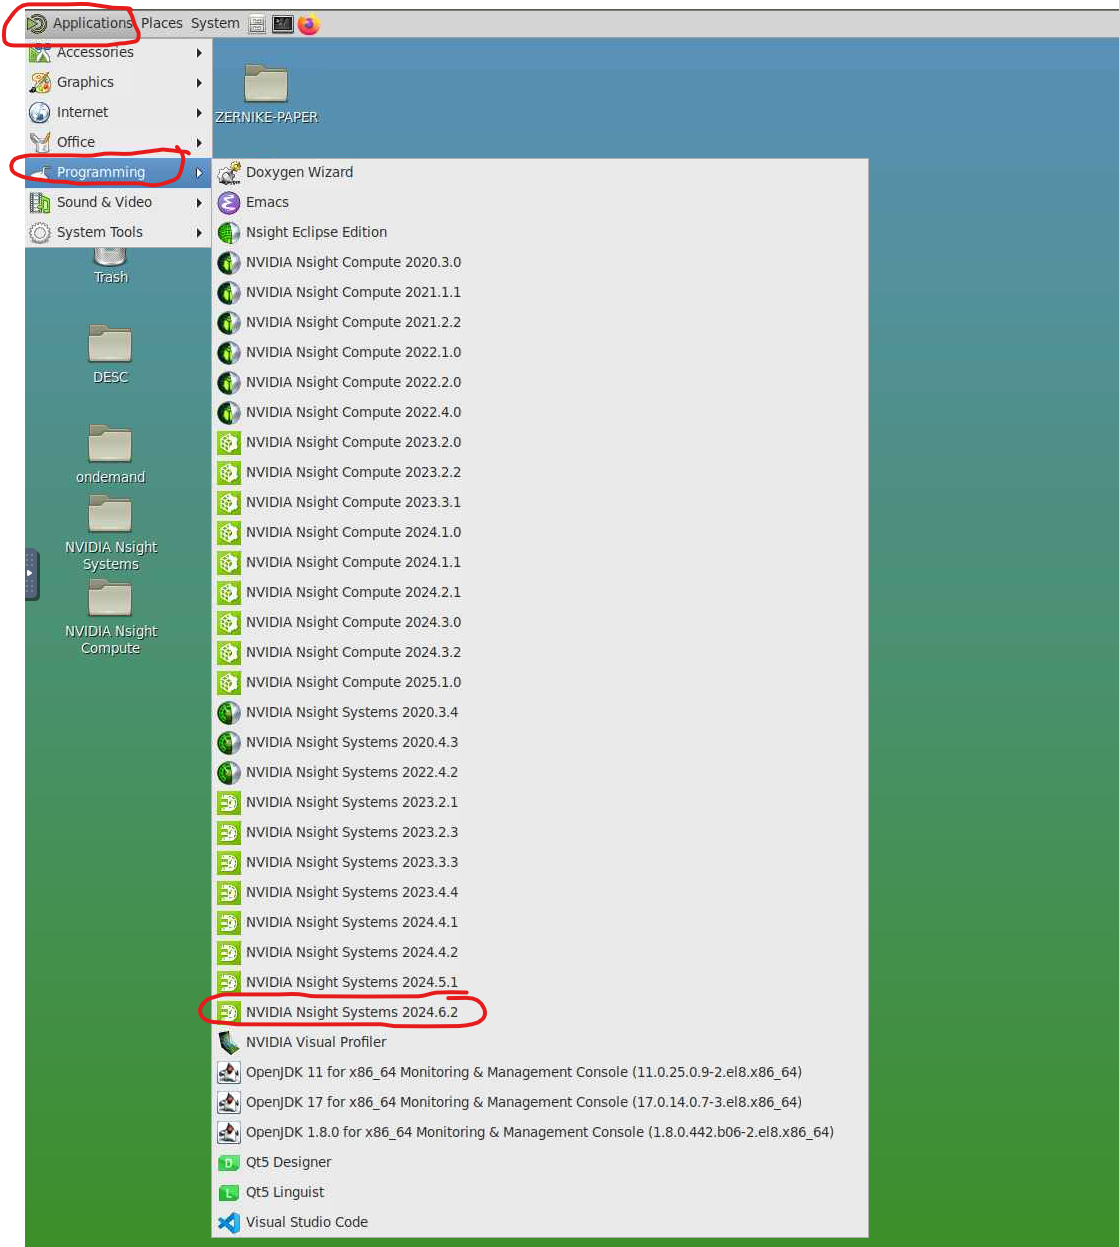
\includegraphics[width=0.5\linewidth]{figures/nsight-systems.png}
\end{figure}
Here is an example report, created for perturb function,

\begin{figure}[H]
    \centering
    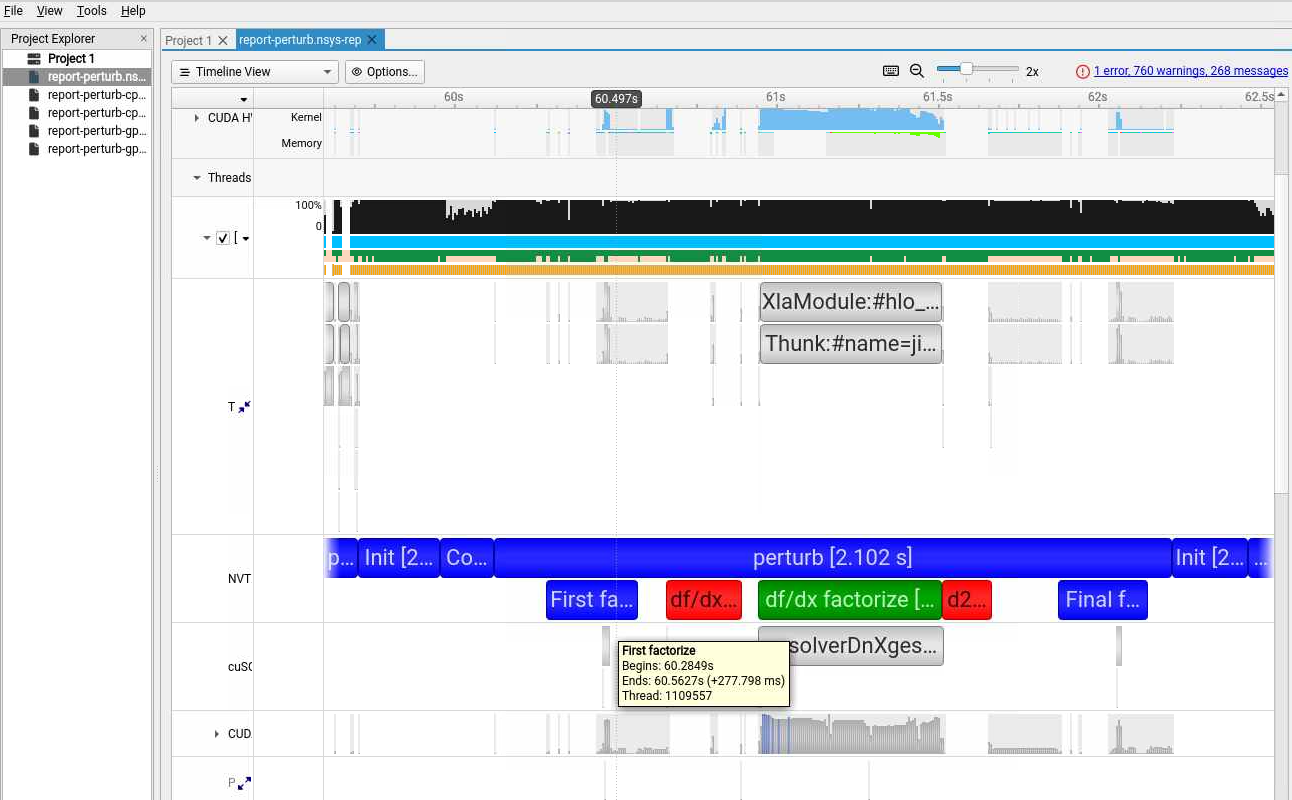
\includegraphics[width=\linewidth]{figures/example-report.png}
\end{figure}

Note that you can add \textbf{nvtx} annotations inside the source code to profile specific places of the code. Unfortunately, you cannot annotate inside a jitted function. However, you can temporarily disable jit and profile like that.

\subsection{Memory Profiling}

Jax by default preallocates 75\% of the available memory to the Jax process.

\begin{minted}[fontsize=\footnotesize]{bash}
XLA_PYTHON_CLIENT_ALLOCATOR=platform
\end{minted}

This will disable JAXs memory preallocation and force it to use CUDAs allocator: while slower, it does make it easier to understand where memory is being allocated, especially when combined with the  \textbf{--cuda-memory-usage=true} option to \textbf{nsys} profile.

See \href{https://jax.readthedocs.io/en/latest/gpu_memory_allocation.html}{Jax documentation}.

Tracing
Instrument code with (\href{https://nvtx.readthedocs.io/en/latest/index.html}{NVTX page})

Recommended to use \textbf{--trace=cuda,nvtx,cusolver} with \textbf{nsys} profile
JAX uses cuSOLVER for the linear algebra operations
Set the option jax.config.update("jax\_traceback\_in\_locations\_limit", -1) 
This will give deeper XLA traces (\href{https://github.com/NVIDIA/JAX-Toolbox/blob/main/docs/profiling.md#tuning-jax-configuration-for-profiling}{see Jax documentation}) 

Starting and stopping instead of profiling the whole app

These functions start and stop the profiler, add them to the top of the file where you want to control profiling:

\begin{minted}[fontsize=\footnotesize]{python}
# profile stuff
import nvtx
from ctypes import cdll
libcudart = cdll.LoadLibrary('libcudart.so')

def cudaProfilerStart(enabled=True):
    if enabled:
        libcudart.cudaProfilerStart()

def cudaProfilerStop(enabled=True):
    if enabled:
        libcudart.cudaProfilerStop()
\end{minted}

And then cudaProfilerStart where you want the profile trace to start. Add cudaProfilerStop where you want the profile trace to stop, or it’ll end automatically at the end. When using start or stop add 
--capture-range cudaProfilerApi
To the nsys profile command otherwise it’ll keep profiling the whole application
Goals for the hackathon

Memory profiling (Can’t get any useful info from Perfetto or NSight. Maybe use tensorboard on a TPU to get an idea? Is there another software or any way to learn memory consumption on a GPU?)
Try float32 or bfloat and see what parts can work with mixed precision
Sharding? It’s not like a shared-data neural network. Instead we have multiple objectives that use the same data (sort of). We want to split the objectives and share the same equilibrium data.
Splitting objectives over multiple GPUs (Scaling tests?)
Writing a small bit of code in native XLA (bad idea, last resort)



Things to try

Call nvidia-smi from different modules inside DESC
Install pynvml pynvml
pip install pynvml
In python code
\begin{minted}[fontsize=\footnotesize]{python}
    import pynvml
    # Initialize
    pynvml.nvmlInit()
    
    …
    # get device handle 
    nvml_handle = pynvml.nvmlDeviceGetHandleByIndex(<device id>)
    …
    # get total memory usage (as seen in nvidia-smi)
    all_mem_gb = pynvml.nvmlDeviceGetMemoryInfo(nvml_handle).used / (1024.0 * 1024.0 * 1024.0)
\end{minted}

Here is an example script we use to look at the memory consumption,
\begin{minted}[fontsize=\footnotesize]{python}
#!/usr/bin/env python3
import subprocess
import time
import threading
import matplotlib.pyplot as plt


def monitor_vram(duration, interval, vram_usage_list, timestamps):
    end_time = time.time() + duration
    while time.time() < end_time:
        result = subprocess.run(
            ["nvidia-smi", "--query-gpu=memory.used", "--format=csv,noheader,nounits"],
            stdout=subprocess.PIPE,
        )
        output = result.stdout.decode("utf-8").strip()
        vram_usage = int(output.split()[0])
        vram_usage_list.append(vram_usage)
        timestamps.append(time.time())
        time.sleep(interval)


if __name__ == "__main__":
    duration = 200  # duration to monitor in seconds
    interval = 0.1  # interval between checks in seconds
    vram_usage_list = []
    timestamps = []

    # create threads for monitoring VRAM and running GPU code
    vram_thread = threading.Thread(
        target=monitor_vram, args=(duration, interval, vram_usage_list, timestamps)
    )

    # start the threads
    vram_thread.start()

    # res = 15
    # run without blocking (Popen)
    # subprocess.Popen(['python', "DESC_profiler_new.py", "5"])
    subprocess.Popen(["python", "DESC_profiler_eq_solve_w7x_mem.py"])

    # wait for the thread to finish
    vram_thread.join()

    # write the VRAM usage to a file
    with open("yge_vram_usage.txt", "w") as file:
        for usage in vram_usage_list:
            file.write(f"{usage}\n")

    plt.figure(figsize=(15, 7))
    # plot the VRAM usage
    times = [t - timestamps[0] for t in timestamps]
    import numpy as np

    vram_usage_list = np.array(vram_usage_list)
    times = np.array(times)

    # this is kind of ad-hoc way of clipping the intended section
    idx = np.where(vram_usage_list > 1000)
    idx = np.arange(len(vram_usage_list))

    plt.plot(times[idx], vram_usage_list[idx], "-or", ms=2)
    plt.xlabel("Time (s)", fontsize=20)
    plt.ylabel("VRAM Usage (MiB)", fontsize=20)
    plt.xticks(fontsize=20)
    plt.yticks(fontsize=20)
    plt.title("GPU VRAM Usage Over Time")
    plt.grid(True)
    plt.tight_layout()
    plt.savefig(f"yge_test0_maxiter2_qr.png", dpi=1000)
    # plt.show()
\end{minted}